\documentclass[12pt]{article}

\usepackage[english]{babel}
\usepackage[utf8x]{inputenc}
\usepackage{pdfpages}
\usepackage{lastpage} % Required to determine the last page for the footer
\usepackage{extramarks} % Required for headers and footers
\usepackage{graphicx} % Required to insert images
\usepackage{listings} % Required for insertion of code
\usepackage{courier} % Required for the courier font
\usepackage{color}
\usepackage{grffile}
\usepackage{float}

\usepackage[a4paper, total={6in, 8in}]{geometry}

% Margins
\topmargin=-0.45in
\evensidemargin=0in
\oddsidemargin=0in
\textwidth=6.5in
\textheight=9.0in
\headsep=0.25in
\fboxsep=0mm%padding thickness
\fboxrule=2pt%border thickness

\linespread{1.1} % Line spacing

\newcommand{\Title}{Vision and scope document} % Assignment title
\newcommand{\Class}{Cos\ 301} % Course/class
\newcommand{\pd}{Post-Doctoral}
\newcommand{\ssr}{Soft\color{green}{Serve }\color{black}}
\newcommand{\version}{1.0}
\newcommand{\iteration}{1}
\newcommand{\client}{Ms. Cathy Sandis (UP Research Office)}
\newcommand{\project}{Post-Doctoral Application Management System}
\newcommand{\repo}{https://github.com/mox1990/Project-Postdoc.git}

\begin{document}


\vspace{4em}

\begin{center}%

\begin{figure}[ht!]
\centering

\includegraphics{../Images_Docs/logo.png}
\end{figure}
\LARGE \bf \project \\[1em]
\LARGE \bf \Title \\[0.25em]
\large \bf \today\\
\bf Version \version\\
\bf Iteration \iteration\\[0.5em]
\Large \bf Prepared for \client\\
\Large \bf by
\Large {\bf \ssr Group }\\[0.5em]
\LARGE {\bf Group members}\\[0.25em]
\large
Kgothatso Phatedi Alfred Ngako (12236731) \\[0.5em]
Tokologo “Carlo” Machaba (12078027) \\[0.5em]
Mathys Ellis (12019837) \\[8em]

\end{center}%

%\newpage
%{\LARGE \bf Change log}\\[2em]

\begin{center}
\begin{tabular}{|l|p{1.4cm}|p{8cm}|p{2.8cm}|}
\hline
\multicolumn{4}{|c|}{\bf Change log} \\
\hline
 Date & Version & Description &  Person \\
\hline
10/02/2014 & v 0.0 & Original SRS document created. & Mathys Ellis \\
\hline
02/03/2014 & v 0.1 & Added to glossary. & Mathys Ellis \\
\hline
05/03/2014 & v 0.3 & Added Introduction, Vision, Background. & Carlo Machaba \\
\hline
06/03/2014 & v 0.4 & Added open issues. Modified some sections. & Alfred Ngako \\
\hline
06/03/2014 & v 0.5 & Added methodology, scope and limitations. & Mathys Ellis \\
\hline
08/03/2014 & v 0.6 & Added some wrapping to the change log which is now a table. & Alfred Ngako \\
\hline
16/03/2014 & v 0.8 & Did some restructuring and document formatting. & Mathys Ellis \\
\hline
17/03/2014 & v 0.8 & Also added to the glossary. & Mathys Ellis \\
\hline
12/05/2014 & v 0.9 & Created new vision and scope document. Transferred necessary content from old SRS document. Performed editing and restructuring of document. Added exclusions. & Mathys Ellis \\
\hline
16/05/2014 & v 0.95 & Updated use case diagrams and stakeholders. & Mathys Ellis \\
\hline
21/05/2014 & v 1.0 & Added import and export services. Finalised document for first iteration. & Mathys Ellis \\
\hline

\end{tabular}
\end{center}
\newpage
\tableofcontents

\listoffigures
\newpage
\section{Project Repository}
\textbf{\repo}
\newpage
\section{Document description:}

\subsection{Document purpose:}
\vspace{0.2in}
This vision and scope document serves the purpose of providing a detailed overview of the project's scope and its vision as well the goals that SoftServe's Post-Doctoral application management system wishes to satisfy. Further it defines the abstract interaction of stakeholders with the proposed software system. Thus this document serves as a contract between SoftServe and the client, Mrs Cathy Sandis of the DRIS of the University of Pretoria in terms of project scope.

\vspace{0.2in}

\subsection{Documentation methodology}
\vspace{0.2in}
\begin{flushleft}
The documentation and software development methodology used by the project adhere to the guidelines set out by the scrum agile methodology. Thus this document has undergone and will undergo various iterations that may extend or reduce the contents of the document.\\

This document was created using the requirement elicitation techniques and requirement definitions as specified by Klaus Pohl’s book Requirements Engineering: Fundamentals, Principles, and Techniques [Dr.Phol, K., 2010].
The requirements, vision and scope were elicited from the following sources:
\begin{itemize}
	\item Numerous interviews with the client.
	\item On-line research into UP Post doctoral applications.
	\item Correspondence with the UP IT department.
	\item Collecting and analysing various documents such as:
		\begin{itemize}
			\item The initial project request document
			\item Application forms
			\item Renewal forms
			\item CV templates
			\item Approval and recommendation forms
		\end{itemize}
\end{itemize}
\end{flushleft}	

\vspace{0.5in}

\subsection{Document conventions:}
\vspace{0.1in}
\begin{itemize}
\item Documentation formulation tool: LaTeX
\item Modelling language: UML 2.0
\end{itemize}

\vspace{0.2in}

\subsection{References:}
\vspace{0.1in}
\begin{itemize}
\item Dr.Phol, K., 2010, \textit{Requirements Engineering: Fundamentals, Principles, and Techniques}, Springer, Heidelberg.
\item DRIS homepage. [online] Available: \textit{http://web.up.ac.za/default.asp?ipkCategoryID=1630} [Accessed on: 31 March 2014].
\end{itemize}	

\vspace{0.5in}

\newpage
\section{Project introduction}
A Post-Doctoral fellow is a person who conducts research after they have completed their PhD, with the aim of deepening their knowledge in a specific field. The University of Pretoria supports such research opportunities in order to the increase research output of the University. Post-Doctoral fellows who conduct their research at the University of Pretoria do so under the supervision of a staff member of the University and their research may be privately or internally funded. This is a growing field in Universities around South Africa. A lack in the software solutions for the application management of Post-Doctoral fellows has been identified by the SoftServe group. To exploit this opportunity the SoftServe group has proposed the following project.
 
\vspace{0.2in}

\section{Project background}
\vspace{0.2in}
The current Post-Doctoral application and renewal processes are paper based thus there are a number of drawbacks, mainly due to human error. One such drawback is that there is no audit trail when it comes to the input of the different stakeholders involved in approving or declining the applications. Another involves the minutes of Post-Doctoral committee meetings which are often misplaced or typed in an inconsistent manner making it hard to recall what has been discussed in the meeting. These meetings play a critical part in the evaluation of prospective applications and renewal applications thus this is an area of concern. Access to the documents involved in the application process is also a problem since they are usually hard copies that change hands constantly. Thus the process of getting access to the documents is long and tedious if not made impossible, since they run the risk of being lost due to various factors. Reporting on the information of fellows, applications, renewals, etc, as well as even communication with the different stakeholders is also problematic due the current system not begin centralised. Therefore gathering all the information required to generate accurate reports is difficult or even impossible. This is where the client Mrs Cathy Sandis saw a potential area that could be optimised by the implementation of a digitalised system. At this point the SoftServe group was brought into the picture.
\vspace{0.5in}

\newpage
\section{Project vision}
\vspace{0.2in}
The client needs a system which can make the management of the application and renewal processes of Post-Doctoral fellowships more effective, reliable, secure and audit-able. Together the client and SoftServe have envisioned a system that will make use of a centralised user friendly web interface that will be used by the all the stakeholders involved in the application and renewal processes. The system will have various sections that handle the different stages in the various processes. The system will need to automate the transitions between phases by forwarding the required information to the next stakeholder in the process and notifying them via an email notification or equivalent. The system will also need to provide reporting facilities for the information stored by the system. As well as progress tracking with regards to any application or renewal. The system data needs to be centralised to ensure that any information used by system is cohesive and valid for any stakeholder who accesses it. Another feature the system should host is that of archival support so that old data can be retrieved if needed. The system will also need to allow importing and exporting of data in predefined formats. By introducing a digital system that is not paper based, the client hopes that the application and renewal processes will be easier to track and manage.
\vspace{0.5in}

\newpage
\section{Stakeholders}

The stakeholders that will engage or be engaged by the system are listed below:

There are four categories under which stockholders can fall:
\begin{itemize}	
\item System or abstract:
These are stakeholders that represent the system itself and generalized users based on their security roles:
\begin{itemize}
\item \textbf{System} - The actual Post-Doctoral application management system.
\item \textbf{System administrator} - The super user of the Post-Doctoral application management system. This user has universal access.
\item \textbf{Authorised user} - A user that has the necessary security roles to perform the operation.
\end{itemize}
\item External:
These are stakeholders that do not have a PeopleSoft account or are prospective fellows.
\begin{itemize}	
\item \textbf{Prospective fellow} - A person who wishes to renew or apply for a post-doctoral research fellowship.
\item \textbf{Referee} - A person who is identified by a Prospective fellow as a referral.
\end{itemize}

\item Internal individuals:
These are stakeholders that do have a PeopleSoft account and are individual members of staff.
\begin{itemize}	
\item \textbf{Research fellow} - A person who is currently in possession of a fellowship.
\item \textbf{Grant holder} - The person who is a fellow's supervisor and a member of staff at the University of Pretoria. This person is also known as the applicant.
\item \textbf{HOD} - The head of the department of which a Grant holder is a member.
\end{itemize}
\item Internal groups:
These are stakeholders that do have a PeopleSoft account and are a group of staff members.
\begin{itemize}	
\item \textbf{Dean's office} - The dean and deputy dean of the faculty under which the department which a particular Grant Holder is a member of. In some cases this may be the dean and deputy dean of research for that faculty if the faculty provides such a responsibility.
\item \textbf{DRIS} - The department of Research and Innovation Support at the University of Pretoria. This stakeholder oversees the application and renewal processes.
\item \textbf{Post-doctoral committee} - The committee who evaluates any post-doctoral fellowship applications and renewals.
\item \textbf{CSC} - The client service centre of the University of Pretoria.
\item \textbf{Finance} - The department of finance at the University of Pretoria.
\end{itemize}
\end{itemize}
\vspace{0.5in}

\newpage
\section{Project Scope:}
\vspace{0.2in}
	
The scope of the project is to design an Post-Doctoral application management system in the form of a software package where prospective fellows can apply for fellowships and current Post-Doctoral research fellows can renew their fellowships at the University of Pretoria. The system will further allow the management of such applications or renewals till the end of the application process. The end is defined as follows: When the DIRS have approved the application and have notified the CSC and Finance department or when the application has been denied and the prospective fellow does not restart the process. The system will replace the current paper based system currently in place. The system will be designed so to allow for future integration with the current student and personnel management system, PeopleSoft, employed by the University of Pretoria. Though the scope of this project will be to construct the proposed system independently of any other system and allow it to run as a stand-alone system.
\vspace{0.2in}

\subsection{Use cases:}

\begin{figure}[H]
\centering	
\framebox{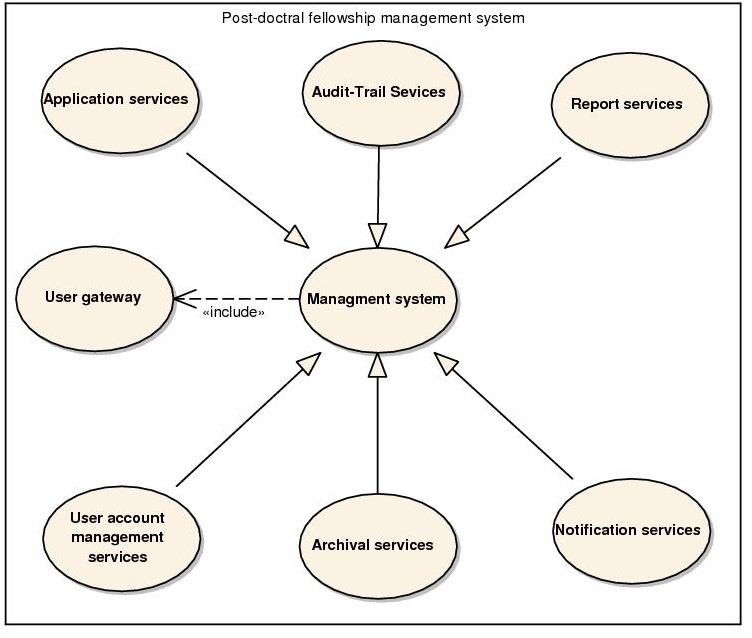
\includegraphics[scale=1]{../Images_Docs/Diagrams/Post-doctral fellowship management system.jpg}}
\caption{Use case diagram of Post-doctoral fellowship management system}
\end{figure}

\begin{figure}[H]
\centering	
\framebox{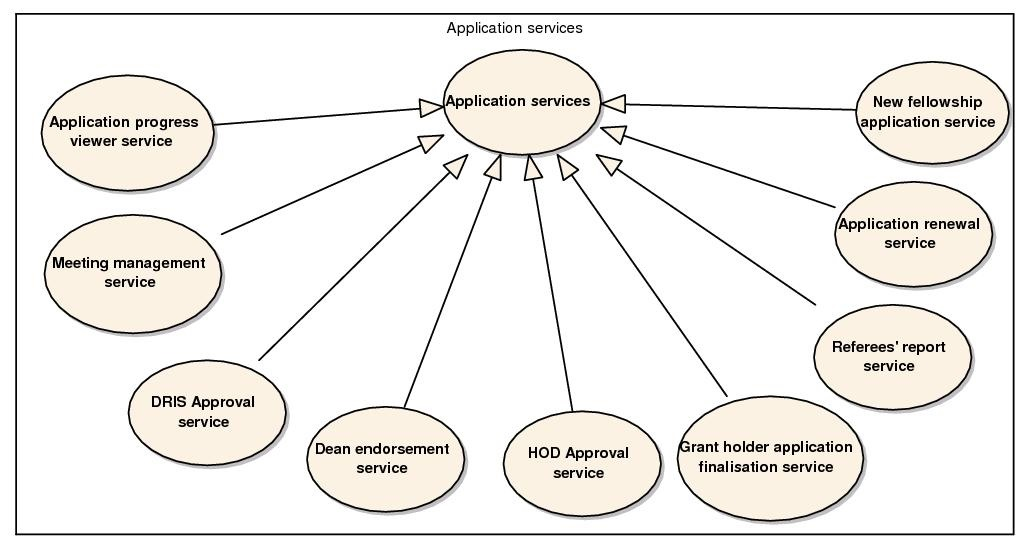
\includegraphics[scale=0.8]{../Images_Docs/Diagrams/Application services.jpg}}
\caption{Use case diagram of Application service}
\end{figure}

\begin{figure}[H]
\centering	
\framebox{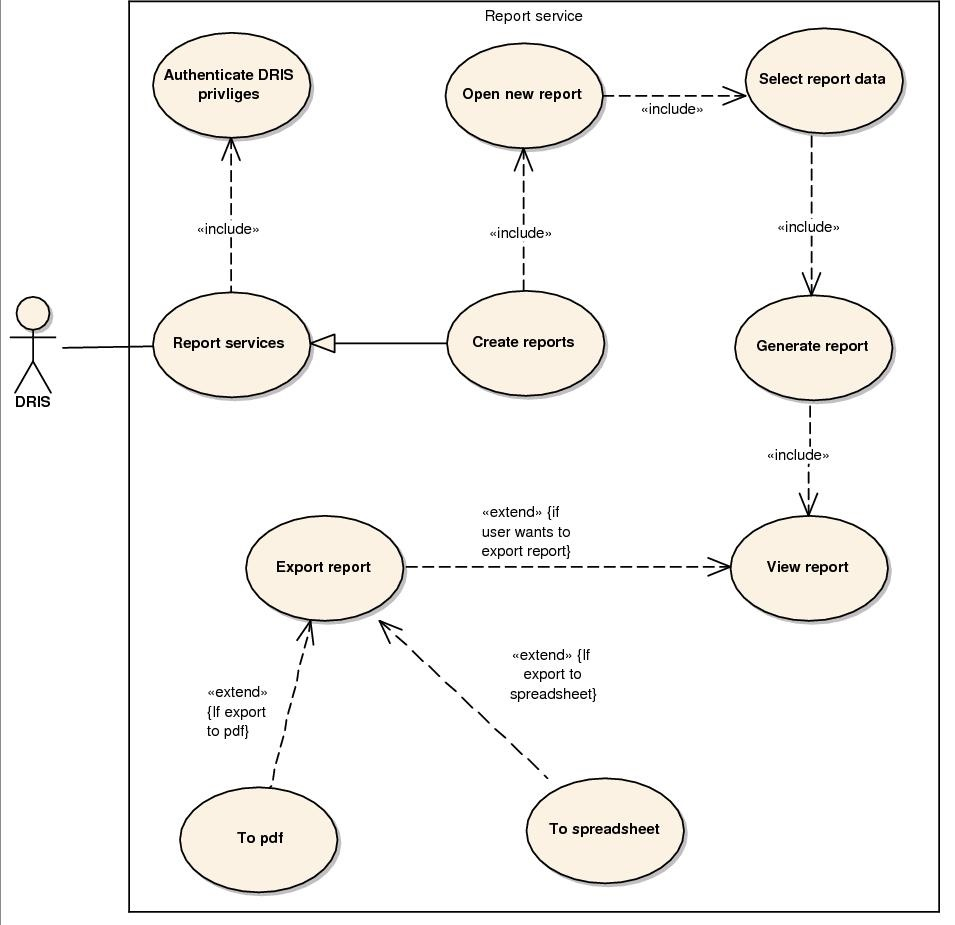
\includegraphics[scale=0.75]{../Images_Docs/Diagrams/Report services.jpg}}
\caption{Use case diagram of Report service}
\end{figure}

\begin{figure}[H]
\centering	
\framebox{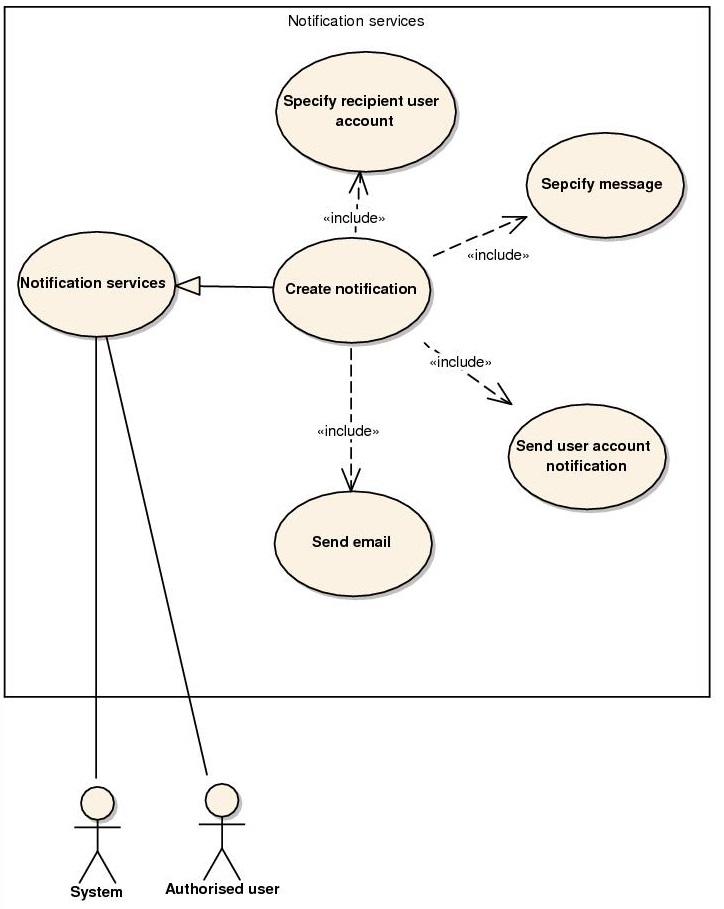
\includegraphics[scale=0.75]{../Images_Docs/Diagrams/Notification services.jpg}}
\caption{Use case diagram of Notification services}
\end{figure}

\begin{figure}[H]
\centering	
\framebox{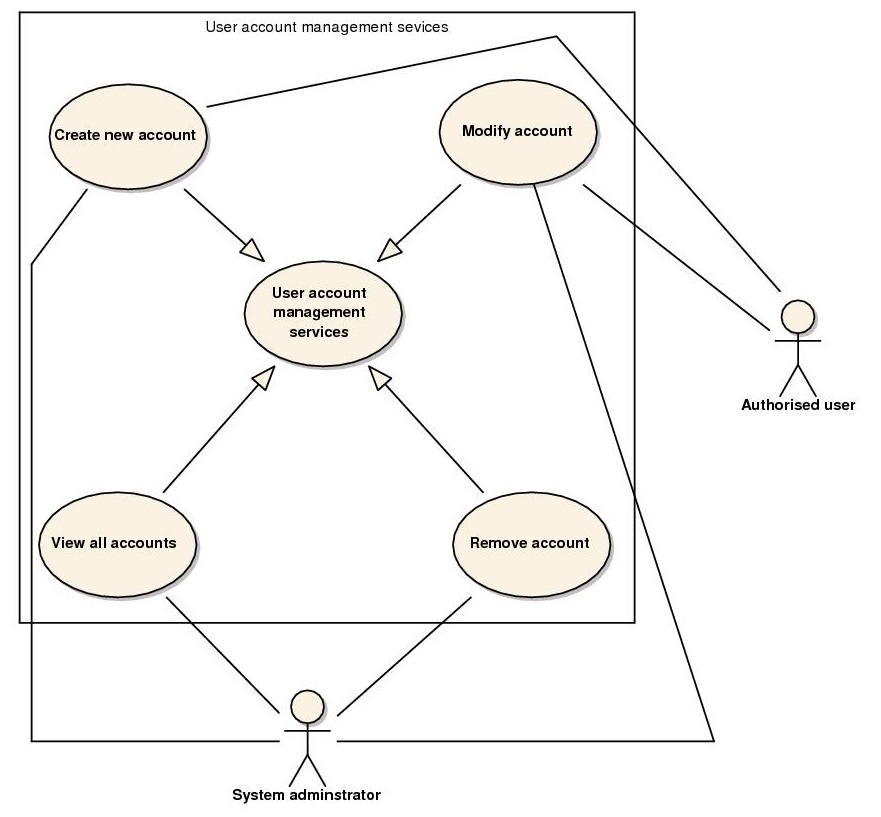
\includegraphics[scale=0.75]{../Images_Docs/Diagrams/User account management services.jpg}}
\caption{Use case diagram of User account management services}
\end{figure}

\begin{figure}[H]
\centering	
\framebox{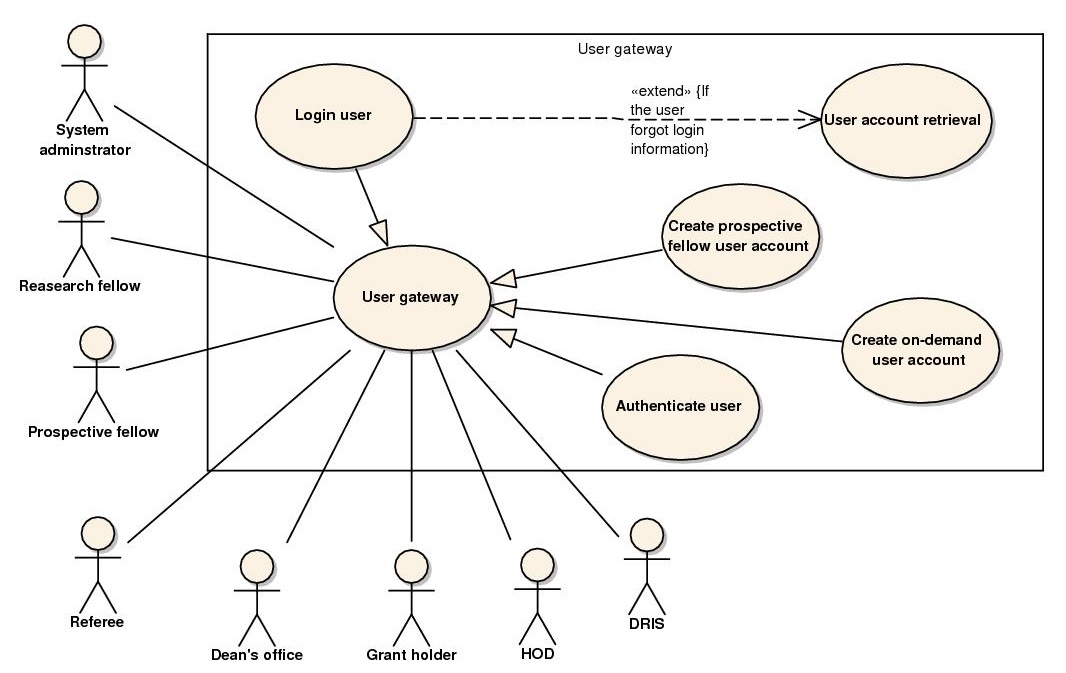
\includegraphics[scale=0.75]{../Images_Docs/Diagrams/User gateway.jpg}}
\caption{Use case diagram of User gateway}
\end{figure}

\begin{figure}[H]
\centering	
\framebox{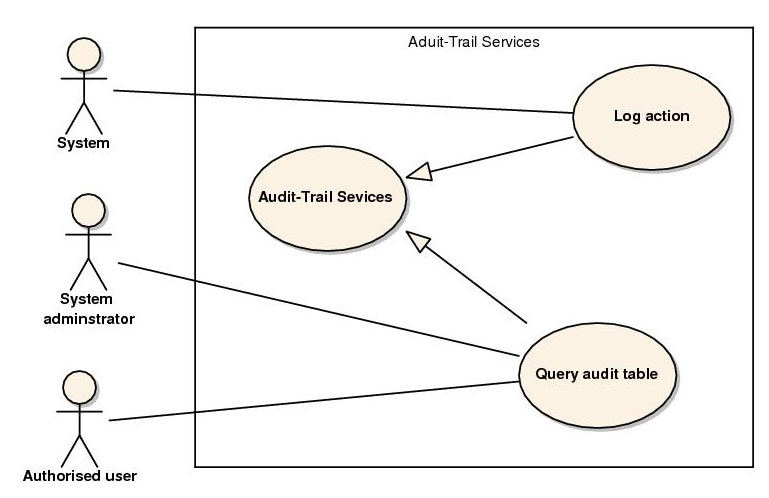
\includegraphics[scale=1]{../Images_Docs/Diagrams/Audit-Trail services.jpg}}
\caption{Use case diagram of Audit-Trail services}
\end{figure}

\begin{figure}[H]
\centering	
\framebox{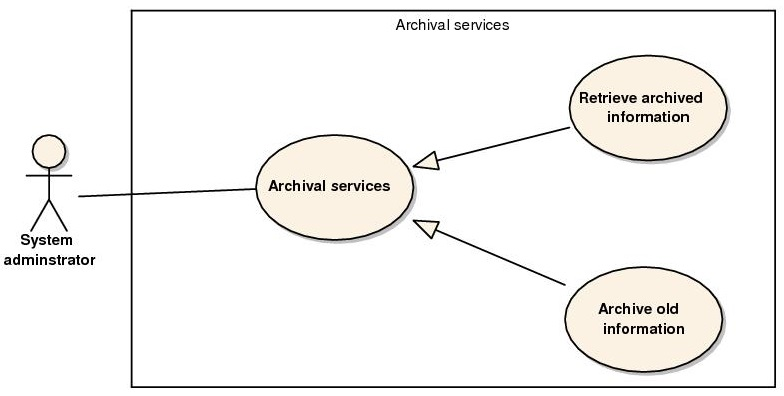
\includegraphics[scale=1]{../Images_Docs/Diagrams/Archival services.jpg}}
\caption{Use case diagram of Archival services}
\end{figure}

\begin{figure}[H]
\centering	
\framebox{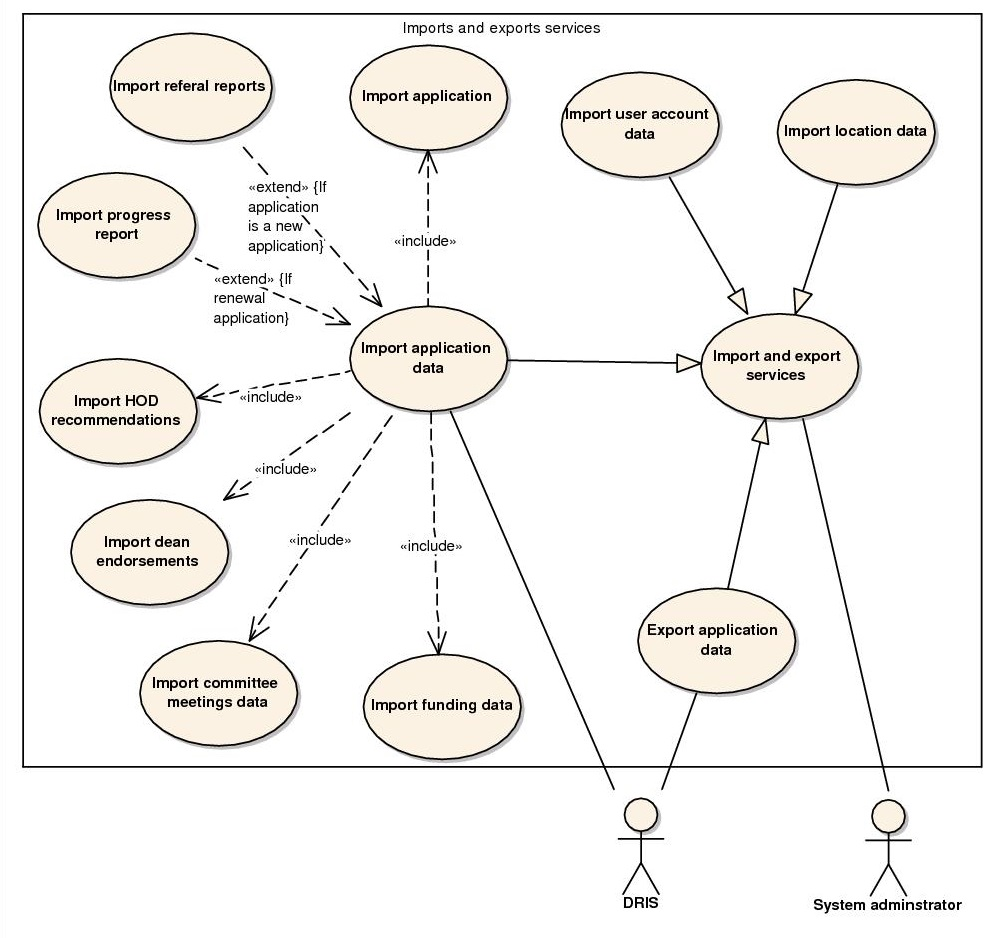
\includegraphics[scale=0.8]{../Images_Docs/Diagrams/Imports and exports services.jpg}}
\caption{Use case diagram of Imports and exports services}
\end{figure}

\vspace{0.2in}
\subsection{Limitations}
\vspace{0.2in}
At the time of writing the project is only limited with regards to the integration with the UP network and the UP's current student and personnel management system. This is due to the IT department of UP only being willing to offer these services or knowledge once the project has been successfully completed. But the system will be developed in such a way to consider the known integration requirements, which at this stage is still very limited.

\subsubsection{Exclusions}
\vspace{0.2in}
Everything not included in this document in terms of scope is considered not in the scope of the project. Though due to the Agile methodology that is employed by the project the scope may be extended or reduced in later iterations if approved by the client.
\vspace{0.2in}

\newpage
\section{Glossary:}
\vspace{0.2in}

\begin{itemize}

\item \textbf{API} - Application Programming Interface
\item \textbf{Application} -Both renewal applications or new fellowship applications are seen as applications by this project.
\item \textbf{CV} - Curriculum Vita
\item \textbf{HTML} - Hyper Text Mark-up Language
\item \textbf{Java EE} - Java Enterprise Edition
\item \textbf{NRF} - National Research Foundation
\item \textbf{PhD} - A doctoral degree in a particular field of study.
\item \textbf{PDF} - Portable Document Format file
\item \textbf{Spreadsheet} - A special type of digital document that is used to represent data in rows and columns
\item \textbf{Use case} - A visual depiction of a service or group of services.
\item \textbf{UP} - University of Pretoria
 


\end{itemize}	

\end{document}